\documentclass[11pt, a4paper]{article}

\usepackage[english]{babel}
\usepackage[utf8x]{inputenc}
\usepackage{amsmath}
\usepackage{mathtools}
\usepackage{amssymb}
\usepackage{amsthm}
\usepackage{graphicx}
\usepackage{subcaption}
\usepackage[colorinlistoftodos]{todonotes}
\usepackage{mathtools}
\usepackage{float}
\usepackage{enumerate}
\author{Marc Cardús, Carla Diví, Arnau Escapa and Enric Sarlé}
\date{\today}

\title{Visualization - Task 4}

\begin{document}
\maketitle
\section{Task description}

In this last task we can freely choose to do the visualization we prefer with the objective of showing what we have learned in this course.

\medskip
The task we have chosen is a dashboard about the NBA statistics data. We have chosen a dashboard visualization because dashboards are composed of several charts and they offer good possibilities to put into practice  the perception principles and users analysis seen in class.

\medskip
The task consists in the following. Imagine that a digital newspaper asks us to create a web page where the user can quickly analyze the performance of their favorites NBA teams. The newspaper also tells us that the user should be able to get the impression of the trajectory of the teams during the last decades ass well with the last season performance.   

\section{Data description}
The data consists in a set of rows of basketball teams by season performances.  For each row there are 61 different features, that be can divided between numerical, categorical and ordinal.

\medskip
Some important columns are the name of the team, the year of the season and the league where the team play. The rest of columns are statistics about the different game aspects. We drop all the rows that does not belong to NBA teams or that are from before 1970. The reason we do so is because we are assuming the user  client is interested in the team trajectories. To show this is enough to use data of the last decades. 



\section{Functional analysis}
In order to fulfill the goals of our digital media clients  and design ideal task structure and information flow with the aim of solving their goals we do a functional analysis.

\subsection{User analysis}

In this case the users are the readers of the digital newspaper. Our hypothesis is that the readers that click into the dashboard page are people interested in NBA. Hence they are familiar with the very basics of the game statics but not necessarily experts of the game.

Regarding to visualization expertise, we can not expect high level of expertise in visualization from the users. Hence the plots must be self-explanatory and easy to understand. The objective is that the charts give a general impression of the performance of the teams without need of analyzing the data they contain  in detail.

\subsection{Task analysis}

We divided the task users in the following ones:

\begin{itemize}
\item Being able to select the desired team in a easy way.
\item Being able to visualize the performance along the lasts decades of the selected team.
\item Being able to visualize the performance of the last season of the selected team and conclude whether it is a good season or not.

\end{itemize}

\section{Data encoding}
In order to achieve a more meaningful data representation of our objectives we combined some our data features.

\medskip
The different game statics (i.e points, rebounds, fouls, assists, etc.) are given as an accumulated value for  a season and team. This are big numbers that  are hard to contextualize for the user. For example, it is hard to extract any information from the fact that a team scores 21232 total points in a season. However the average points per game is an easier  information to precess since the user is familiar with this range of data. For example if we say that a team scores 70'3 points per game, the user may know it is a low value because the usual scores in basketball are higher.
\medskip

However, we are not assuming that the users are experts on the field so one of the objectives of the charts is that we show this information in a way that is easy to detect weather they are hight values or not without expert knowledge.

\medskip

In a similar way that the game statics we converted the different number of made and missed shots into made shots percentages. (for each kind of shots: field goals, free throws and three points).






\section{Representational Analysis}

We design the dashboard with the aim of giving a solution to  the tasks listed in the functional analysis taking into account the capabilities of the user. Taking this into account we designed different charts that will compose the dashboard.
\medskip

At the top of the dashboard the user will be able to select a team by using a button that displays a list of the teams when clicking it. When a team is selected we show its logo in order to help its recognition.

The rest of the dashboard consist in a set of charts that display their information depending on the team selected. They are distributed in two main parts: in the left of the dashboard the charts show information that is meant to encode the trajectory of the team in the last decades the right side is meant to infer weather the team had a good season in the last year.
 
\subsection{Teams trajectory charts}

This part of the dashboard is composed by two charts: a line chart and a bar chart. The goal of this plots is that the user can perceive the tendency of the team taking into account their history.

\medskip
The bar chart compares the number of wins and loses along the last 40 years. We show wins and losses because the number of games may change due to lockout. The line chart shows the number of wins distinguishing into away and home games in the last 40 years.

\subsection{Current season charts}
This part of the dashboard is divided in two parts: a radar chart and 3 donuts charts. The objective of this plot is show the characteristics of the team in the current season.

\medskip

In the radar chart we show the team average by  game  of the most important match statistics: rebounds, assists, turnovers, steals and personal fouls. In order to interpret weather the values are good or not we compare them with the average by game statistics of the opponents when facing the selected team. In this way the user can know with a quick look weather the selected team achieves more assists (i.e any other feature) than its rivals.

\medskip

We decided not to add points and blocks to the radar  because the range of this features are two high for points and two low for blocks. If we added the points the differences in the other features would not have been perceivable. The differences in blocks are not high enough to be interesting. 

\medskip

Donuts charts show an important sadistic in basketball: percentage of made shots. We do one small donut chart for each of the types of shots of the game: field goals, three point shots and free throws.

\subsection{Pencil prototype}

We consider that it can be useful to create a pencil prototype before going into D3 so that there were no misunderstandings with the definitions of the charts. 
\bigskip
\begin{figure}[H]
\centering
%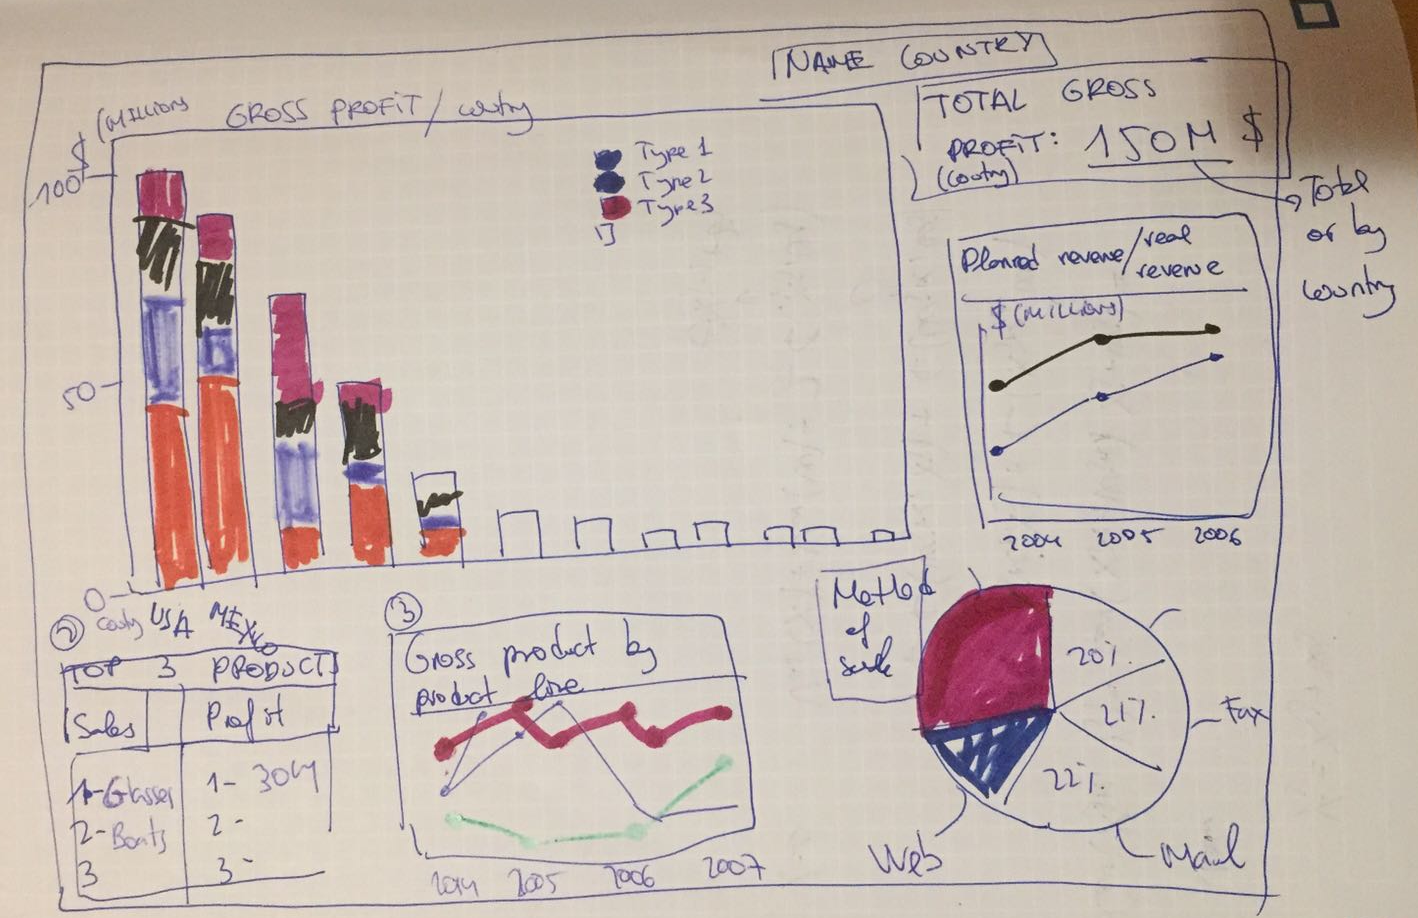
\includegraphics[width=0.78\textwidth]{pencil.png}
\caption{Pencil prototype}
\end{figure}

\section{Duties for member}

Our methodology consists in allocating of tasks and weekly Skype meetings to integrate and discuss. We would like to point out that we have worked as a team, and everyone helped each other along the project. 

\medskip
First part, designing the product:
\begin{itemize}

\item Data description and functional analysis. Arnau Escapa 

\item Product design. Full team brainstorming 
\end{itemize}
Second and most time consuming part, coding.
\begin{itemize}
\item Trajectory. Carla Diví  and Marc Cardús
\item Current Season. Enric Sarlé and Arnau Escapa
\item Integration. Full team efforts.
\end{itemize}


\section{Further improvements}
This is a list of different things that we wish we could had done better but we couldn't because of lack of time and/or html coding skill.
\begin{itemize}
\item Re-adjust the charts automatically. (only size of dashboard windows is automatically adjusted).
\item Transitions when changing a team. 
\item Show information about the best players of each team.
\item When displaying the list of teams show their logo.
\end{itemize}
\section{References}
\begin{itemize}
\item Source of the data set: https://www.kaggle.com/open-source-sports/mens-professional-basketball/data
\item Dashboard structure: https://github.com/keen/dashboards
\item Plots: class notes and https://www.bl.ocks.org

\end{itemize}
\section{Final overview}
Just in case the browser affects to the overview. This is how we see it:

\bigskip
\begin{figure}[H]
\centering
%\includegraphics[width=1.15\textwidth]{overview.png}
\caption{Final overview of the dashboard}
\end{figure}
\end{document}
